
\documentclass[11pt]{article}

\usepackage[square,sort,comma,numbers]{natbib}

\bibliographystyle{abbrvnat}
\setcitestyle{authoryear,open={(},close={)}}
\usepackage[utf8]{inputenc}
\usepackage{epsfig}
\usepackage{latexsym}
\usepackage{hyperref}
\usepackage{graphicx}
\usepackage{tikz}
\usetikzlibrary{shapes.geometric, arrows}
\DeclareGraphicsExtensions{.pdf,.png,.jpg}
\begin{document}
	
	\title{Research Proposal}
	
	\author{Nirbhay P. Tandon\\MSc. Data Science\\
		Research Title:\\Develop New Transformer Architecture For \\ Question \& Answering(Q\&A)
	}
	\date{}
	\maketitle
	
	\newpage
	\begin{abstract}
		Attention-based Transformer architectures have become the norm of current Natural Language Processing applications. Google began this trend back in 2017 with their paper \textit{Attention Is All You Need}, by introducing the Transformer architecture that works solely on attention mechanisms. The purpose of our work will be to explore a new kind of Transformer architecture. Compare \& contrast its performance against other architectures such as BERT, DistilBERT, ALBERT etc. that are also based on SQuAD 2.0 Dataset. Through our research, we aim to produce a new Transformer Architecture that has a better performance than existing models for Question Answering in a conversational manner.
	\end{abstract}
	\newpage
	\tableofcontents
	\newpage
	\listoffigures
	\newpage
	\section{Introduction}\label{introduction}
	
	Question-Answering based systems have gained a lot of popularity, especially in the form of "chatbots". These systems depend highly on contextual understanding of the input, the training corpus \& the question asked. They use this knowledge to output an answer that can help the user with whatever their query is. Recurrent neural networks and architectures based on them, have been able to provide great advancements in the field of Question-answering \& chatbots in general. However, there is a behaviour of over-fitting \& lack in contextual understanding of the question. This, coupled with long training times \& extremely complex mathematical model designs, have often kept the field of Natural Language Processing slightly obscured from the masses. 
	\\
	We wish to change that. Through our work, we would like to aim at creating a sustainable, fast, easy to understand Transformer architecture for the purpose of Question Answering. An advancement on the work done by the team at Google  \citep{atayl}.
	
	We have divided our research proposal into 7 sections.
	In Section \ref{introduction}, we shall take a look at briefly introducing the concept \& why our work is necessary. Next, in Section \ref{backRR}, we outline the background work that has already been done in this field and how some of the papers relate to the work that has been done. We use this as an opportunity to highlight some of the shortcomings in current architectures \& modelling techniques. In Section \ref{aims}, we briefly outline the aim of our proposed research. In Section \ref{researchMeth}, we define in some detail the work that we will do to establish our research \& how we plan to quantify the work that shall be done. Section \ref{expectedoutcomes}, highlights our goal, which is to produce a new transformer architecture that performs better at Question Answering based tasks \& is capable of doing so in a conversational manner.
	In Section \ref{resources}, we have outlined the minimum hardware requirements along with the resources available to the author. Finally, in Section \ref{plan} we submit a Gantt Chart to outline our plan against the number of weeks.
	
	\section{Background \& Related Research}\label{backRR}
	In this section, we shall highlight why this research has been conducted, what has led us this far \& some of the interesting challenges that it poses. In \ref{back}, we briefly look at the history of Natural Language Processing \& how some of the challenges were addressed. In \ref{rr}, we look at the most interesting \& latest research that has gone into creating the Transformer architecture, identify some of the common patterns \& use that information to strategise our model in other sections.
	\subsection{Background}\label{back}
	The area of Natural language Processing has taken significant leaps in the last two decades. Work was done towards improving the ability of machine learning models to first recognize words, then sentences, followed by contextual understanding has led to several interesting \& novel approaches in the field. From early on neural networks to creating Long Short-Term Memory architectures\citep{originallstm} by Sepp Hochreiter \& Jurgen Schmidhuber helped in the mid-'90s that resolved the vanishing gradient problem of classical neural networks, we have come a long way.
	
	The latest advancements in this field come from Google's research lab in the form of \textit{Transformers}. In their paper Attention Is All You Need\citep{atayl} Vasvani et. al demonstrated how replacing the \textit{encoder-decoder} based recurrent layers with \textit{multi-headed self-attention} based ones removes the need for recurrence and convolutions entirely. We look into this in a bit more detail later.\\
	
	
		
	\subsection{Related Research}\label{rr}
	Outlined below are some of the most important pieces of research in the field of Natural Language Processing based neural networks, long short-term memory architectures \& transformers.
	\begin{enumerate}
		\item The SQuAD 2.0 Dataset by \citep{dataset}, was developed with funding from Facebook to help address some major issues with existing datasets. Key pain points of these being a focus on questions that can be easily answered or use of automatically generated, unanswerable questions which are easily identifiable.\\
		The SQuAD 2.0 dataset resolves this by combining the SQuAD dataset along with 50,000 crowd worker generated unanswerable questions. The most important feature of these being that the unanswerable questions must look similar to answerable ones. For a model to be successful on this new dataset, it must be able to answer all possibly answerable questions as well as determine when no answers are provided for a question in the given paragraph \& abstain from answering. A comparative study done for a natural language understanding task that obtained an 86\% score on SQuAD 1.1, only got 66\% on the new 2.0 dataset.
		The dataset helps bridge the gap between true natural language understanding \& machine understanding by using the concept of Relevance. Through comparisons with various datasets such as RACE, MCTest, QASENT etc. they have identified the missing links like negative examples, antonyms \& helped fill the gap. This dataset forces the models to understand whether a paragraph span has the answer to the question posed. 
		
		\item Work done in the field of Long short-term \& gated recurrent \citep{lstm} \& \citep{recurrent} neural networks, in particular, has been established as a state of the art approach in sequence modelling, transduction problems such as language modelling and machine translation.
		In their paper Attention Is All You Need,\citep{atayl} the team set out to resolve problems in the parallelization \& increased compute times of recurrent models. The inherently sequential nature highlights the issues in memory constraints, leading to reduced batch sizes.
		\begin{figure}[h!]
			\centering
			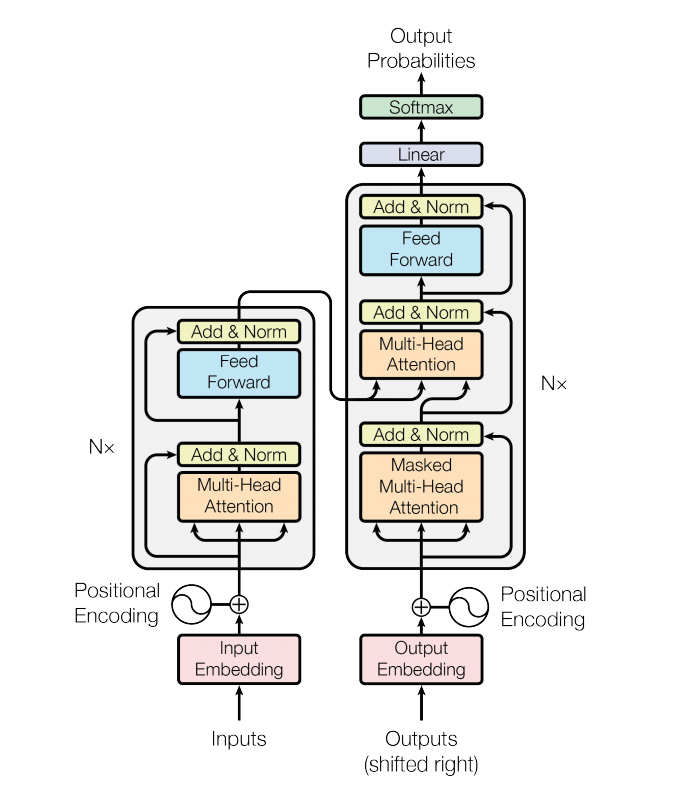
\includegraphics[scale=0.4]{transformer.png}
			\label{fig1}
			\caption{Transformer Architecture built by \cite{atayl}}
		\end{figure}
		The architecture for a \textit{Transformer} in this paper is outlined as having an encoder that maps input sequences to a continuous representation. The architecture can be seen above in Figure 1. This is then decoded into an output sequence of symbols one at a time. Each step is auto-regressive, i.e. it consumes the previously generated symbols as additional input when creating the next. This is similar to an ensemble tree architecture. Stacks of 6 encoder layers \& 6 decoder layers is used.\\
		The encoder layers each have 2 sub-layers of a multi-head self-attention \& the other a simple, position-wise fully connected feed-forward network layer.\\
		The decoder layer is similar to the encoder layer \& has an additional 3rd sub-layer that performs multi-head attention over the output of the encoders. There is also normalization \&  the outputs are prevented from attending to subsequent positions. \\ The attention mechanism can be described as mapping a query to a set of key-value pairs\citep{atayl}. This can bee seen from \ref{fig2}. \\The evaluations performed on the Wall Street Journal dataset\citep{wsj}, using 40k sentences, showed that even without task-specific tuning the model had better results.
		\begin{figure}[h!]
	\centering
	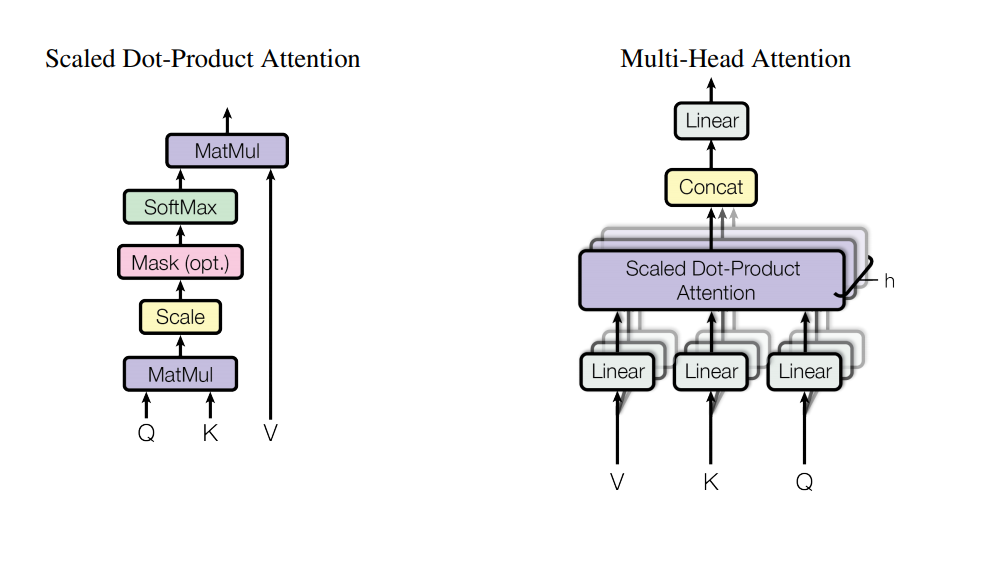
\includegraphics[scale=0.4]{multihead.png}
	\label{fig2}
	\caption{Scale Dot \& Multihead Attention Models\cite{atayl}}
\end{figure}
		\item bert  Language model pre-training has been shown to be effective for improving many natural language processing tasks (Dai and Le, 2015; Peters et al, 2018a; Radford et al, 2018; Howard and Ruder, 2018).
		The two approaches share the same objective function during pre-training, where they use unidirectional language models to learn general language representations. The authors present BERT fine-tuning results on 11 NLP tasks. 4.1 GLUE
		
		The General Language Understanding Evaluation (GLUE) benchmark (Wang et al, 2018a) is a collection of diverse natural language understanding tasks.
		The authors present BERT fine-tuning results on 11 NLP tasks.
		The General Language Understanding Evaluation (GLUE) benchmark (Wang et al, 2018a) is a collection of diverse natural language understanding tasks.
		To fine-tune on GLUE, the authors represent the input sequence as described, and use the final hidden vector where C belongs to set RH, corresponding to the first input token ([CLS]) as the aggregate representation.
		The only new parameters introduced during fine-tuning are classification layer weights W belongs to RKxH, where K is the number of labels.
		Results: The best performing method concatenates the token representations from the top four hidden layers of the pre-trained Transformer, which is only 0.3 F1 behind fine-tuning the entire model.
		This demonstrates that BERT is effective for both finetuning and feature-based approaches.
		Using only the RND strategy performs much worse than the strategy as well
		Conclusion: Recent empirical improvements due to transfer learning with language models have demonstrated that rich, unsupervised pre-training is an integral part of many language understanding systems.
		These results enable even low-resource tasks to benefit from deep unidirectional architectures.
		The authors' major contribution is further generalizing these findings to deep bidirectional architectures, allowing the same pre-trained model to successfully tackle a broad set of NLP tasks. \citep{bert}
		\item fastqa \citep{fastQA}
		\item roberta \citep{roberta}
		\item alert \citep{albert}
		\item distilbert \cite{distil}
		\item schmidhuber \citep{schmid}
		\item levy \citep{levy}
		\item contextual \citep{contextual}
		\item lstm \citep{lstm}
		\item zhang \citep{zhang}
	\end{enumerate}
	
	\newpage
	\newpage
	\section{Aims \& Objectives}\label{aims}
	
	The main aim of this research is to propose a new transformer architecture that can perform better at conversational Question \& Answering from the SQuAD 2.0 dataset\citep{dataset}.
	We shall:
	\begin{enumerate}
		\item Implement the existing models that are available via libraries such as HuggingFace\citep{hfTransformers}, PyTorch \& Tensorflow, run the SQuAD 2.0\citep{dataset}
		\item Obtain F1, validation, etc. scores for existing models \& treat them as our benchmark scores
		\item Identify drawbacks of the current architectures
		\item Design our architecture \& evaluate its performance
		\item Fine-tune the architecture, re-evaluate \& report improvements
		\item Compare the results of our Transformer model with the benchmark scores.
	\end{enumerate}
	We hope to establish our proposed transformer architecture as a competent enough contender to be used within both industry \& academia.
	\section{Research Methodology}\label{researchMeth}
	
	To implement this research we shall break the project down into 5 phases. These are outlined below.
	\subsection{Research Dataset}\label{datas}
	
	We have selected is the Stanford Question Answering Dataset (SQuAD). It was created as a reading comprehension dataset with the help of crowd workers. It is based off of questions posed by these workers on a set of Wikipedia articles, where the answer to every question is a segment of text, or span, from the corresponding reading passage, or the question might be unanswerable \citep{dataset}.
	
	The dataset consists of over 150,000 questions. Split into 100,000 answerable \& over 50,000 unanswerable question, that were written by crowd workers to look similar to unanswerable questions. The challenge being that a model should be able to correctly answer the answerable questions \& abstain from answering the unanswerable ones. In their paper \textit{Know What You Don't Know: Unanswerable Questions for Squad}, \cite{dataset} the authors have described how they 
	The dataset is freely available as a part of the Transformers package in python or it can be downloaded from the SQuAD 2.0 website \citep{squad}.
	
	To effectively use this dataset for our purposes, let us first take a look at what its contents look like below.\\ \\
	\noindent\fbox{
	\parbox{\textwidth}{\textbf{Context: } \textit{"The Normans (Norman: Nourmands; French: Normands; Latin: Normanni) were the people who in the 10th and 11th centuries gave their name to Normandy, a region in France. They were descended from Norse ("Norman" comes from "Norseman") raiders and pirates from Denmark, Iceland and Norway who, under their leader Rollo, agreed to swear fealty to King Charles III of West Francia."}\\	
		\textbf{Question: } \textit{Who was the Norse leader?}\\
		\textbf{Answer: } \textit{Rollo}}
	}
	\\ \\
	
	The answer of the aforementioned question is quite simple for humans to comprehend. The challenge is for us contextualize this \& make it machine understandable, so that our model can answer it correctly.
	
	The dataset consists of various kinds of English language examples like negation, antonyms, entity swaps, impossible conditions to answer, answerable, etc. making the dataset a well balanced one. 
	
	To use this dataset correctly we shall perform the following pre-processing steps on it:
	
	\begin{enumerate}
		\item Data splitting into separate Question, Answer \& Context lists.
		\item Splitting the data into separate training \& validation sets of  question \& answers using the 80/20 rule, also known as the Pareto principle. We will have 80\% training data \& 20\% test data.
		\item Tokenization of the split data to generate "context-question" pairs
		\item Generating indexes for when an answer begins \& ends in the dataset
		\item Adding answer tokens based on their encoded positions
	\end{enumerate}	
	\subsection{Research Benchmarks}\label{benchmarks}
	Here we shall focus on obtaining benchmark scores for the shortlisted architectures i.e BERT \citep{bert}, DistilBERT \citep{distil} \& Albert \cite{albert}, on the above dataset \citep{dataset}. 
	
	We shall use the F1, Exact Match \& Accuracy scores to determine if our model has performed better or not.
	
	\subsection{Architecture Creation}\label{architecturecreation}
	In this section we will:
	
	\begin{enumerate}
		\item{Mathematically model a new transformer architecture}
		\item{Code the architecture}
		\item{Run sample dataset to identify base benchmarks}
		\item{Run the SQuAD 2.0 dataset\citep{dataset} to obtain 1st pass performance benchmarks}
		\item{Document architecture performance, identify pros \& cons}
	\end{enumerate}
	\subsection{Architecture Refinement}\label{refinement}
	In this phase, we will focus on:
	\begin{enumerate}
		\item{Reviewing the results from the previous section}
		\item{Identifying the areas of improvement}
		\item{Hypothesise the improvements \& implement them in the architecture}
		\item{Run the SQuAD 2.0 dataset\citep{dataset} to obtain new performance benchmarks}
		\item{Document architecture performance, identify pros \& cons}
	\end{enumerate}
	\subsection{Model Evaluation}
	The training shall be carried out on each of the models for 100 epochs. We shall also look at the specificity/recall of these results to better understand if our work was done correctly or not. F1, accuracy, recall, specificity
	\section{Expected Outcomes}\label{expectedoutcomes}
	
	We expect that our created model is at-par, if not better performing than existing models for Question Answering based problems.
	\section{Requirements \& Resources}\label{resources}
	
	To successfully deliver on our research we will be utilizing the following hardware:
	\begin{itemize}
		\item EVGA GeForce RTX 2070 SUPER KO GAMING, 08G-P4-2072-KR, 8GB GDDR6, Dual Fans\citep{evga}. This graphics card is based on the Nvidia "Turing" architecture \& has 2560 CuDA cores.
		\item Intel 10700 processor. 8 cores, 16 threads, 16M cache\citep{intel}.
		\item VENGEANCE® LPX 8GB (1 x 8GB) DDR4 DRAM 2400MHz C14 Memory Kit - Black\citep{Ram}. 8GB x 4, 32 GB total.
		\item Ubuntu 20.04 Operating System
		\item We will also be using the latest versions of the following packages: Pandas, NumPy, SciPy, Transformers by HuggingFace, Matplotlib, Tensorflow \& PyTorch. In case there are compatibility issues the appropriate versions will be mentioned. We will also mention any other packages that might be required in the course of the research.
	\end{itemize}
	
	
	The above hardware is available to the author \& any changes to the same will be notified/highlighted in the subsequent reports.
	\section{Research Plan}\label{plan}
	
	Shown on the next page is the Gantt Chart highlighting the research stages \& timelines.\\
	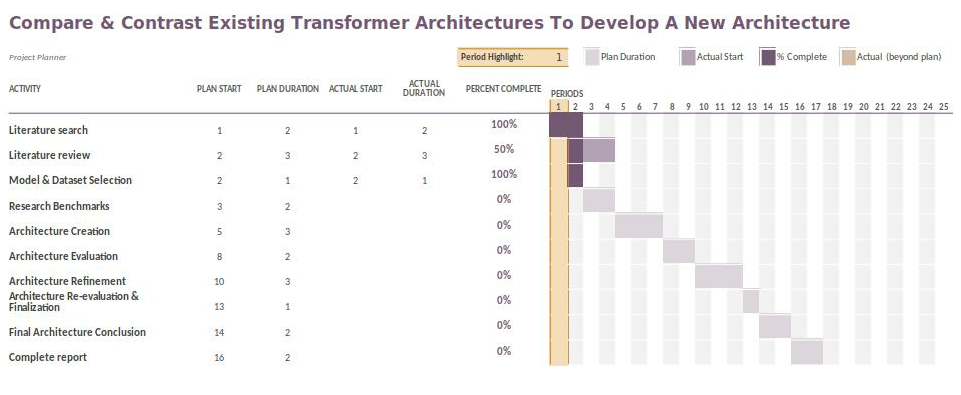
\includegraphics[width=180mm,height=120mm,angle=90]{g2.png}
	\newpage
	\bibliography{Research_Proposal}
	
\end{document}
